\documentclass[sigchi, review]{acmart}

\usepackage{booktabs} % For formal tables

% Copyright
\setcopyright{none}
%\setcopyright{acmcopyright}
%\setcopyright{acmlicensed}
%\setcopyright{rightsretained}
%\setcopyright{usgov}
%\setcopyright{usgovmixed}
%\setcopyright{cagov}
% \setcopyright{licensedcagov}
%\setcopyright{cagovmixed}
%\setcopyright{licensedothergov}

% DOI
\acmDOI{10.475/123_4}

% ISBN
\acmISBN{123-4567-24-567/08/06}

%Conference
\acmConference[CHI'19]{ACM SigCHI conference}{April 2019}{ElPaso, Texas USA}
\acmYear{2019}
\copyrightyear{2019}

\acmPrice{15.00}
\usepackage{CJKutf8}

\usepackage{multicol}
\usepackage{multirow}
\usepackage{array}
\usepackage{booktabs}
\usepackage[utf8]{inputenc}

\begin{document}
\begin{CJK*}{UTF8}{gbsn}

\title{A Conceptual Framework of Delay Perception in 3D Tele-Immersion}

\titlenote{Produces the permission block, and copyright information}
\subtitle{Extended Abstract}
\subtitlenote{The full version of the author's guide is available as
  \texttt{acmart.pdf} document}

\author{Leave Authors Anonymous}
\affiliation{
  \institution{Institute}
  \city{City}
  \state{Country}
}
\email{example@email.com}

\author{Leave Authors Anonymous}
\affiliation{
  \institution{Institute}
  \city{City}
  \state{Country}
}
\email{example@email.com}

\author{Leave Authors Anonymous}
\affiliation{
  \institution{Institute}
  \city{City}
  \state{Country}
}
\email{example@email.com}

% The default list of authors is too long for headers.
\renewcommand{\shortauthors}{B. Trovato et al.}

\begin{abstract}

3D Tele-Immersion (3DTI) allows distributed users to communicate in a same virtual space. It grows rapidly in recent years. However, few works were conducted to study user experience in 3DTI. Delay is an important factor that affects user experience. In this paper, we explore users' perception of network delay in 3DTI. We propose a conceptual framework that levels delay requirements of 3DTI tasks into three classes: \emph{synchronous} tasks, \emph{audiovisual} tasks and \emph{visual Only} tasks. \emph{synchronous} tasks involves interactions at the same time, e.g., instrument ensemble and the Rock-Paper-Scissors game. They require a low delay of 30 $\sim$ 100 ms. We suggest that 3DTI supports much more tasks of this delay-sensitive level compared to the 2D situation. The other two levels are common in 2D, e.g., teleconference and playing chess. We suggest that they require a delay of 200 ms or more in 3DTI. The requirement is lower because the users are less sensitive and more tolerable to delay in 3D. We describe an example study to illustrate our framework. For each level, the framework gives suggestions of network engineering to save network resources and improve the user experience.

\end{abstract}

%
% The code below should be generated by the tool at
% http://dl.acm.org/ccs.cfm
% Please copy and paste the code instead of the example below.
%
\begin{CCSXML}
<ccs2012>
<concept>
<concept_id>10003120.10003121.10003126</concept_id>
<concept_desc>Human-centered computing~HCI theory, concepts and models</concept_desc>
<concept_significance>300</concept_significance>
</concept>
</ccs2012>
\end{CCSXML}

\ccsdesc[300]{Human-centered computing~HCI theory, concepts and models}

\keywords{Delay perception; 3D tele-immersion}

\maketitle


\section{Introduction}

The last century has witnessed the development of telecommunication from telegram, telephone to multimedia, which has been dramatically and continuously reshaping our lives and human society \cite{friedman2007world}. Behind this, a trend of growing richness in telecommunication techniques is also manifest. From text, audio to video, it points to human beings' essential need of communicating in an immersive way \cite{apostolopoulos2012road}. Recently, profiting from the rapid development of GPUs and head-mounted displays (HMDs), 3D telepresence (e.g., Holoportation \cite{orts2016holoportation}) has again been attracting people's attention. 3D telepresence builds on real-time 3D reconstruction, transmission, and rendering of people and the entire space. This new telecommunication paradigm is considered to represent the highest level of immersion in telecommunication.

% Recently, benefit from the head-mounted displays (HMDs) 3D tele-immersion technology (e.g. Holoportation \cite{orts2016holoportation}) arises and satisfies such an envision of highest level of immersion [XX]. A 3DTI system can reconstruct the scene in real-time and transmit the result to remote so that remote users can interact with. 

%owning to the progress in real-time 3D reconstruction and rendering technology.

%Recently, the development of VR/AR  (display) and sensing (stereo camera), computing (3D construction) has made 3D tele-immersiveness into reality. 

The unique and core benefit of a 3D telepresence system is the sense of "co-presence": remote participants can interact with each other as if they present "in the same space at the same time" \cite{orts2016holoportation, kraut2003visual}. For example, remote users in two distributed sites can see each other, visually shake hands, share the same space and the same object as if they were face-to-face in the real world. Due to the rich information shared between sites in real-time, 3D telepresence enables a substantial set of novel and promising applications that cannot be achieved before, such as remote chess games, dance collaboration, and piano duet. Meanwhile, 3D telepresence also creates a tremendous research space in the area of Human-Computer Interaction, where many research questions deserve to be studied, such as human factors, user behavior, collaboration techniques, and so on.

% [NOTE] image quality改成percieved rendering quality,因为前者属于QoS。和quality of experience (user experience)同级的topics还可以有user's ability,user's behavior等等。

% 3DTI can enable face-to-face human-to huamn interaction with co-present sense. This would provide a new platform for research QoE and interaction techniques. 

%The engineering difficulties involve all aspects on sensors, hardware and software.

However, currently, developing and deploying a 3D telepresence system is challenging and requires masses of resources. For example, to support a single site, Holoportation \cite{orts2016holoportation} deployed 24 industrial cameras and five distributed PCs. The challenge even concerns more on the development aspect. First, generally speaking, the core algorithms of 3DTI builds upon considerable knowledge and expertise of mathematics and computer graphics that cannot be acquired easily. Second, the engineering part involves quite a number of model parameters and hardware acceleration designs (i.e. CUDA), which directly impacts the performance but are seldom reported in the research paper. The high cost of building a 3DTI system impedes HCI research in this area in the first place. 

% [错误] First, although 3D reconstruction is a well researched area, works on real-time 3D reconstruction are relatively few and new (summarized in Section 2).

% 然而,目前来说,开发和部署1套3DTI系统的成本和资源花费是很大的。这个不仅仅是硬件成本问题,比如holoportation用了32 cameras 和 4 pcs来覆盖一个空间,更多的还是背后技术实现问题。首先,在这个领域,虽然3D construction研究很多,但是如何做到real-time的研究工作较少也比较新。一般来说,3DTI系统的核心算法涉及到涉及到大量的数学,计算机图形学的专业知识。而且在实际实现过程中,还会存在着大量的参数设置和硬件加速优化等诸多工程问题。这些都细节都没有正在文章中公开,但是对于性能有着重要影响。而我们认为开发和部署的高成本很大程度上阻碍了hci研究在这个问题上的发展。

% However, the cost of developing and deploying 3DTI is extremely high, which impedes research in this area at the first place.  For example, Holoportation [XX] not only used dozens of industrial camera and distributed PCs. More importantly is the algorithm. 软件部分总体上就是数学上复杂,代码量巨大,算法细节不公开(比如在holoportation中需要对non-rigid body进行tracking,tracking技术往往需要调整很多参数,才能得到好的质量),实现细节不公开(比如这是一个以访存为瓶颈的GPU工程,其中的访存结构,steaming顺序,都会极大地影响pipeline的效率). 3DTI researchers needs to spend a lot of resource to build it. 

% to reconstruct the 3D model of both the surrounding and users in real time, each site was equipped with 24 cameras (16 Near Infra-Red cameras and 8 color cameras) and 4 PCs, with each using two NVIDIA Titan X GPUs. In addition, the algorithm builds on sophisticated pipeline which cannot be acquired without an expertise on computer vision and CUDA developing. The reconstructed model was transmitted to a dedicated dual-GPU fusion machine for rendering over a point-to-point 10Gbps network. Finally, Holoportation provided an end-to-end latency of 80ms, and an average error of 3 millimeters at 1 meter distance and 6 millimeters at 1.5 meter distance. Even though, the performance still does not satisfy the requirement as indicated in previous research in 2D [XX, XX]. Other systems It has both financial and human cost to develop such a system. 
% However, the cost of developing and deploying 3DTI is extremely high, which impedes research in this area at the first place. The engineering difficulties involve all aspects on sensors, hardware and software. For example, in the implementation of Holoportation [XX], to reconstruct the 3D model of both the surrounding and users in real time, each site was equipped with 24 cameras (16 Near Infra-Red cameras and 8 color cameras) and 4 PCs, with each using two NVIDIA Titan X GPUs. In addition, the algorithm builds on sophisticated pipeline which cannot be acquired without an expertise on computer vision and CUDA developing. The reconstructed model was transmitted to a dedicated dual-GPU fusion machine for rendering over a point-to-point 10Gbps network. Finally, Holoportation provided an end-to-end latency of 80ms, and an average error of 3 millimeters at 1 meter distance and 6 millimeters at 1.5 meter distance. Even though, the performance still does not satisfy the requirement as indicated in previous research in 2D [XX, XX]. Other systems It has both financial and human cost to develop such a system. 

% [NOTE] which impedes \textbf{HCI} research in this area.
% sensors, hardware and software --> hardware, pipeline and algorithm. 
% 我个人觉得这一段说holoportation的缺点,有点过长了。虽然能够很现实地说明他们存在的问题,但是这样写(过分强调他人不足)可能会引起一部分人的反感。另外,其实他们硬件贵的地方是很surprise的,主要来自24个工业摄像头(这里就需要几十万)。也许我们应该直接指出来,不然别人还以为是贵在NVIDIA Titan X了,而一个Titan其实只需要一万元左右。10Gbps network和显卡还是少提为妙,因为其实我们也用了的同等级的设备。他们的delay可以说,误差可以不说,他们的误差做得比我们厉害得多。
% 重要:computer vision --> computer \textbf{graphics}

%Current, the average error of 3 millimeters at 1 meter distance and 6 millimeters at 1.5 meter distance.  The end-to-end latency is 80ms. The final result of Holoporation and its shortcomings in supporting the applications, especially about the latency that exceeds the requirement of communication according previous research in 2D [XX, XX]. 

% However, currently, building such a platform is expensive. How Holoportation did it, in what cost? Even with Holoportation, there still lacks balance. It cannot satisfy all requirements. We think lack a platform present the first and basic obstacle to promote research in this area. 

The aim of our work is to provide a low-cost and easy-to-deployment 3DTI system, based on which HCI researchers can easily build up 3DTI applications and conduct user research. The system should wrap the core algorithms mentioned above and provide easy-to-use APIs that HCI researchers are familiar with. As a result, HCI researchers can focus their effort on implementing the desired interaction or effects. We are also planning to open source the system, so that others can contribute to the underlying algorithms or functions. Our ultimate goal is to advance 3DTI research in HCI community. 

% Given computing resource is always the bottleneck, the key is to identify the impact of individual performance metric (e.g. latency and image quality) on the quality of user experience, and then take most advantage of the limited computing resource to optimize the most important metrics. 
% To achieve this, compromise has to be made so that although some experience metric may be sacrificed, but the most important one are supported. This requires identification of critical design metrics that compete on the computing resource and a deliberate balance between performance requirements.
To inform the design of the system, we first brainstormed 9 representative applications in 3DTI. We then refer to prior literature on QoE (quality of experience) in telecommunication, and analyze their performance requirement accordingly. We finally identify two core requirements, \textit{high synchronicity} and \textit{shared props}, which underline the importance of temporal synchronization and spatial alignment to ``co-presence'' user experience in 3DTI respectively: 
%first analyze the requirements. We perform a brainstorming about potential applications in 3DTI, which serve as the basic set to be parsed. We analyse their features (which highligths the co-presence experience as a priority to image quality) and combine with QoE research in 2D, we sacrifice the rendering solution, and set several design goals that make up the ``co-presence'' and implications for 3DTI, highlight the spatial and temporal definition of ``co-presense''. We summarize as three aspects:

% 供参考:我在这方面稍微有点怂。如果我们过于强调我们牺牲了渲染质量来换取响应能力和交互特性,可能会引起3DTI专家的反感(不知道reviewer里会不会有这样的人),因为渲染质量恰恰是3DTI里很难做而且我们的确没做好的事情。不如从正面写,我们支持了low-cost,low delay,支持了co-presence中的方方面面,同时渲染质量也不差(用户能够接受)。

\begin{itemize}
 \item \emph{high synchronicity}: The system should reach a low network delay to meet the high synchronicity of some tasks, e.g., shaking hands and dancing together. The high synchronicity is one of the basic requirements of co-presence \cite{kraut2003visual}.
 
 Why it is important?
 \item \emph{shared props}: Shared props is a component of co-presence. It allows users to interact with distributed physical objects that looks like one shared prop. The reconstruction algorithm supports shared props by merging similar objects. Physical shared objects provides common grounds that are important for the communication \cite{luff1998mobility, kraut2003visual}.
%  \item \emph{augmenting physical objects}: Physical objects can be augmented to other prop in the virtual space. For example, an iPad can be augmented as a piano or a keyboard.
\end{itemize}

% Based on these systems, we develop a 3DTI system to reflect the design goals, and finally present the finally implementation reference. The system basic information. low-cost, easy-to-development add-ons. Our final system requires 1 PC at each site with four depth cameras for capturing. The cost 7000\$ for two sites. The project is open-sourced and readily to be used by others. 
% Based on the requirements above, we design and implement our 3DTI platform. 
Our final 3DTI system meets the need of HCI research in three aspects. First, the system fulfills the two core requirements of co-presence. It reaches a one-way network delay as low as 50 ms, and supports shared props with an accuracy of XX mm. The systems run in 30 frames per second, and provides acceptable rendering quality. Second, the system is low-cost to deploy. It consists of inexpensive commercial devices, including 2 RealSense and 1 PC on the source site, and a head-mounted displays (HTC Vive) on the remote site, which costs \$7000 in total. Third, our system is released as a Unity3D plugin, so that developers can build upper-layer applications by taking advantage of rich resources in Unity3D. This makes the development easy and efficient.

% It provides a sync assistance for delay-sensitive tasks. 

% The system enables changes on physical objects by using Virtual Reality (VR).

% A drawback of our system is the relatively low rendering quality. However, we deem that it is acceptable for a HCI research.

To assess the effectiveness of our system, we conducted two user studies. The first focused on the \textit{high synchronization}. We developed a Rock-Paper-Scissors game to test the latency requirement of the highest level in 3DTI. Results showed that a one-way network latency of 50ms was not easily noticed by users, and could well satisfy the QoE requirement in 3DTI. 
% In addition, we propose a mechanism to compensate the experience if network latency cannot be avoided. 
In the second user study, we studied the user experience enabled by \textit{shared props} in the fully co-present situation. We built a chess game, where participants in each site interacts with a physical chessboard and the chess pieces of their own side. Participants reported a strong sense of co-presence provided by the system. The two studies together validated the design and implementation of our system. 

\vspace{2mm}

In sum, the contributions of this work are three-fold: 
\begin{itemize}
\item We provided a systematic review and analysis of 3DTI technologies and QoE requirements, which informs the design and implementation of future systems. 
\item We provide a low-cost and easy-to-deploy 3DTI system, which is open sourced. Developers can build 3DTI application easily and efficiently in popular commercial IDE (i.e. Unity3D). 
\item We evaluated the effectiveness of our system with two user studies, which also provided valuable empirical results as well as insights into the user experience of 3DTI applications. 
\end{itemize}

% In conclusion, our work contributes in the following: 

% \begin{enumerate}
% \item an analysis of the design requirements of 3DTI given low-cost solution. 
% \item an implementation of the system which is open-sourced. 
% \item an evaluation that validate the system and also gives insights on the benefit of co-presence research. 
% \end{enumerate}

% The past centuries have witnessed the growth of communication technology. The invention of the telephone has saved a great deal of time and money by displacing physically face-to-face meeting. Higher levels of immersion is a tendency. Several new communication techniques emerged in the past two decades, such as teleconference \cite{allen1996teleconferencing, marlow2016beyond}, telecollaboration \cite{donovan2014understanding, avellino2015accuracy}, robotic telepresence \cite{jouppi2001robotic, misawa2015chameleonmask, neustaedter2016beam}, and so on.

% 3DTI allows distributed users to communicate and interact with each other in the same virtual space. It is the tele-communication with the highest level of immersion so far. 3DTI grows rapidly in the past decade \cite{kurillo2008immersive, petit2010multicamera, maimone2011encumbrance, maimone2012real}. Both the improvement of pipeline and hardware make 3DTI hopeful to be practical in the near future. Microsoft's Holoportation \cite{orts2016holoportation} is a typical 3DTI pipeline with high-quality and real-time performance. For computing, GPUs are getting more powerful. For rendering, immersive displays such as Head-Mounted Displays (MHDs) are becoming popular.

% Prior works on 3DTI mainly focus on technical implementation. Researchers tended to improve the quality of 3D reconstruction and rendering through dedicated devices and complex pipelines. Most 3DTI systems are not open-source, not easy to deploy and do not support easy application development. This phenomenon leads to a high threshold that hinders the research of HCI in 3DTI. As a result, the interaction requirements of 3D have not been well discussed yet. For example, many example tasks in prior 3DTI systems is possible in 2D communications [?, ?, ?].

% In this paper, we aim at a lightweight and open-source 3DTI system that provides convenience for HCI research. The system should be easy to deploy and at the same time meet the interaction requirements of 3D. To explore the requirements, we brainstormed possible tasks in 3DTI. Based on these tasks, we identified three requirements of our system:

% \begin{itemize}
%     \item \emph{high synchronicity}: The system should reach a low network delay to meet the high synchronicity of some tasks, e.g., shaking hands and dancing together.
%     \item \emph{co-present and shared props}: Co-present is an important concept in 3DTI that users feel like exactly at the same place. Furthermore, some tasks require shared props, e.g., the shared chessboard in a remote chess game.
%     \item \emph{modifying physical objects}: Physical objects can be modified to improve interactions in the virtual space \cite{lindlbauer2018remixed}. For example, two iPads in distributed places can be fused into a virtual piano so that two users can play piano duet.
% \end{itemize}

% Based on the requirements above, we design and implement our 3DTI system. The advantages of our system is twofold. First, the system is easy to deploy. It consists of inexpensive commercial devices (\$7000 in total). The project is open-source and can be released as an Unity3D plugins, which provides convenience for application development. Second, the system meets the interaction requirements explained above. It reaches a one-way network delay of 50 ms. It provides a sync assistance for delay-sensitive tasks. The system uses Head-Mounted Displays (HMDs) to support co-present. The reconstruction algorithm supports shared props by merging similar objects. The system enables changes on physical objects by using Virtual Reality (VR). A drawback of our system is the relatively low rendering quality. However, we deem that it is acceptable for a HCI research.

% To validate the practicality of our system, we conducted two user experiments. The first experiment was to test if our system is responsive enough to support a network delay-sensitive task. We applied the Rock-Paper-Scissors game as the task. Result shows that users are satisfied with our system. Furthermore, our sync assistance significantly improved the user experience. The second experiment was a remote chess game. Through observation and interview, we found positive features of the interaction in our system, e.g., users leverage body language to assist their communications; most users can not tell the difference between touchable objects and purely virtual objects.

% % [paragraph] paper structure
% In the remainder of the paper, we first review 3DTI systems in details. We also have a brief review on media richness and synchronicity (section 2). We next discuss the interaction requirements of 3D by brainstorming and analysis (section 3). Next, we introduce our 3DTI system (section 4). Then, we describe the experiment for illustration and validation (section 5). The paper concludes by discussing our limitation and the future work (section 6).

% [abandon] the difference between 2D and 3D
% Despite of the sufficient research in 2D, it is still necessary to rebuild the framework of delay perception in 3D. The reason is the large difference between 2D and 3D. First, 3DTI can support more applications and improve some existing tasks in a more nature manner. We have to discuss them case by case. Second, 3DTI refers to a higher level of immersion, which offers more visual cues. Previous work \cite{tam2012video} have pointed out that video increase users' tolerance to delay. This effect may be enhanced in 3D. Third, the 3DTI systems need a great amount of computing resource and network bandwidth, which calls for higher network requirements and coping strategies.

% [abandon] The importance of studying delay perception.
% Network delay is a crucial problem in communication technology. On the one hand, network delay significantly affects user experience \cite{brunnstrom2013qualinet, schmitt2014asymmetric, schmitt2013qoe, wu2009quality}. For example, the network delay should be within 150 ms to provide a good user experience for audio-mediated communications \cite{recommendation2003114, donovan2014understanding}. On the other hand, new communications generally require higher bandwidth. It challenges the requirement of low network delay \cite{kleinrock1992latency}.

% [abandon] 
% Numerous works explored network delay perception in telephone and 2D communications. However, no work has studies network delay perception in full 3D tele-immersion, i.e., with reconstruction and rendering in full 3D. It is necessary to rebuild the framework of network delay perception in 3D because of the large gap between 2D and 3D. First, 3D environment supports co-present, that is, the two users feel like at the same virtual space. Second, 3D offers much more visual information. These features may lead to unknown changes in network delay perception in 3D.

% [abandon] in this paper, we propose the framework
% In this paper, we explore users' perception of network delay in a full 3D tele-immersion system. We systematically reviewed previous works on network delay perception. We came up with some hypotheses about the problem. To support these hypotheses, we first built a 3DTI system with an ideal network delay of 50 ms and then conducted a controlled study. Finally, we proposed a framework of network delay perception in 3DTI.

%The framework suggests that users perceive network delay by cues. A user perceives the network delay if he feels that his partner response to the cues abnormally, because the perceived response time is prolonged by the round-trip network delay. In previous works, there are three types of cues: synchronous cues, conversation and visual feedback. Among them synchronous cues is the strongest one to reveal network delay, while the visual feedback is the weakest one.

%The framework infers significant changes of network delay perception in 3D. First, more applications fall into the delay-sensitive level \emph{synchronous tasks}. We should pay attention to support their low network delay. Second, users are less sensitive and more tolerable to the network delay in 3D conversations. Based on these findings, we give suggestions for network design.

%  [paragraph] Contributions of our work
%Our contribution is threefold. First, this work explains how users perceive network delay in 3D and infers significant changes in 3D network delay perception. Second, we give suggestions on network design for each situation in 3D. Third, our project is open-source [?]. We give necessary explanations to make sure that the readers can easily build up a similar system.


\section{A Framework of Delay Perception in 3DTI}

%We present a conceptual framework of delay perception in 3DTI. \textbf{In this framework, 3DTI applications are divided into three levels according to their delay requirement. 这句话不清楚,很想知道什么是一个level,但是没有满足预期,猜也猜不到}. Suggestions are given to network engineering for each level. \textbf{Furthermore, we have designed an experiment to illustrate the framework.} Readers can reconstruct the experiment to precisely measure the delay requirement of a specific application.

% The structure of our framework
We present a conceptual framework of delay perception in 3DTI. The framework divides 3DTI tasks into three levels: tasks with \emph{synchronous interaction}, \emph{conversation} and \emph{only visual feedback}. Correspondingly, the three levels of tasks call for high, middle and low requirement of network delay. For each level, the framework also gives suggestions to improve the perceived quality of network.

The framework is supported a comprehensive reviews of previous works. Delay perception is a well-understood research question in audiovisual DIME. \textbf{Our framework partly relies on previous theories and study results(这句话不清楚)}. However, there is a large difference of delay perception between 3DTI and audiovisual DIME. Thus, we take the features of 3DTI into account in order to form our framework.

Noticeability and tolerance of delay are two important factors that were measured by most studies \cite{wu2009quality, schmitt2014influence, geerts2011we, schmitt2014asymmetric}. Some studies also focus on users' perception of overall network quality. These metrics are users' subjective rating in a specific task, and with a specific delay. In our study, we assess subjective feedback via questionnaires similar to \cite{schmitt2014influence}. The questionnaire is on a 5-point Likert scale (Table \ref{tab:table_questionnaire}).

\begin{table} [!htbp]
\begin{tabular}{|p{0.25\columnwidth}|p{0.35\columnwidth}|p{0.3\columnwidth}|}
\hline 
Label & Question & Scale \\
\hline
quality & How do you feel during the experiment? &Bad <--> Excellent \\
\hline
noticeability & Can you perceive the delay in the connection? & Very much <--> Not at all \\
\hline
tolerance & To what extent where you annoyed by the delay? & Severe annoyance <--> No annoyance \\
\hline
\end{tabular}
\caption{Questions and scale.}
\label{tab:table_questionnaire}
\end{table}

A 3DTI developer may expect a certain recommended delay for his application. However, previous works \cite{montagud2012inter} [?, ?, ?] pointed out that delay perception is largely dependent on user differences and context. Thus, we should investigate the noticeable and tolerable boundary of delay, which is statistically suitable for most users. We first refer to a psychology concept called Just Notice Difference (JND) \cite{xu2013exploiting, sat2009statistical}:

\begin{itemize}
    \item \emph{JND}: With other variables fixed, the value for which 50\% of the subjects perceive a difference in their quality.
\end{itemize}

Most related studies recommend using \emph{noticeable delay} and \emph{tolerable delay} as certain values in discussion. We define them as follows:

\begin{itemize}
    \item \emph{Noticeable Delay}: the threshold delay that most users can just perceive. In our experiment, we define it as the 50\% JND of zero delays, i.e., more than 50\% of participants score 1 point for noticeability.
    
    \item \emph{Tolerable Delay}: the threshold delay that most users can just tolerant. In our experiment, we define it as the just intolerable delay minus its 50\% JND, i.e., less than 50\% of participants score 4 or 5 points for disruptiveness.
\end{itemize}

We illustrate the relationship between noticeable delay and tolerable delay in figure xxx.

The noticeable delay is very insightful for network engineering. On the one hand, developers should try to improve the network service, to reach the noticeable delay. On the other hand, when a service is already within noticeable delay, we can appropriately increase the delay to have more room for smoothing or recovering packet loss \cite{xu2013exploiting}.

[NOTE] Tolerable delay indicates a boundary that is nearly intolerant. An application can not simply target at it, because it is already a bad service. Instead, the tolerable delay can be used to assess the Quality of Experience (QoE). [?] suggests a linear correlation between end-to-end delay and user experience. We can use noticeable delay and tolerable delay to determine the correlation.

[NOTE from zsyzgu] Here I change my mind about the tolerant delay. Delay can be perceived by cues for sure, however, the tolerance of delay in a specific task may depend on much more factors such as fairness and interactivity \cite{ishibashi2006subjective, montagud2012inter}. So we are not going to model the tolerant delay anymore, but list factors to affect it according to previous work. We will also introduce a way to measure tolerance of a specific delay in a specific task, in our example experiment.

We next introduce the three synchronization levels. The basic idea is the observation that user perceive delay by cues. We determine the level of a task by judging if it contains cues of \emph{synchronous interaction}, \emph{conversation} and \emph{visual feedback} 这个是按照什么来分的?看关键词感觉不到维度. As Table \ref{tab:table_synchronization_levels} shown, we recommend their noticeable delay and tolerable delay by summarizing previous audiovisual works and adapting to the 3D situation (从audiovisual adapt到3D的策略和原则是什么?).

\begin{table} [!htbp]
\newcommand{\tabincell}[2]{\begin{tabular}{@{}#1@{}}#2\end{tabular}}
\begin{tabular}{|p{0.25\columnwidth}|p{0.2\columnwidth}|p{0.2\columnwidth}|p{0.2\columnwidth}|}
\hline 
\textbf{Levels} and \emph{Examples} & Noticeable Delay & Tolerable Delay & 3.5 MOS \\

\hline
\textbf{Synchronous Interaction} & \textbf{20 - 50 ms} & \textbf{50 - 100 ms} & ?? ms \\
\hline
\emph{Rock-Paper-Scissors} \cite{hashimoto2006influences} & 40 ms & ?? ms & 70 ms \\
\hline
\emph{Virtual car driving} \cite{pantel2002impact} & 50 ms & 200 ms & ?? ms \\
\hline
\emph{example} [?] & ?? ms & ?? ms & ?? ms \\

    
\hline
\textbf{Conversation} & \textbf{100 - 150 ms} & \textbf{300 - 400 ms} & ?? ms \\
\hline
\emph{3D Visual Communication} \cite{wu2009quality} & 120 ms & ?? ms & ?? ms \\
\hline
\emph{Video Group Discussion} \cite{schmitt2014asymmetric} & 500 ms & 1000 ms & 500 ms \\
\hline
\emph{Audiovisual telecommunication} \cite{tam2012video} & ?? ms & ?? ms & 500 ms \\
\hline
\emph{Take turns reading random numbers aloud as quickly as possible} \cite{kitawaki1991sub} & ?? ms & ?? ms & 80 ms \\
\hline
\emph{Take turns verifying random numbers as quickly as possible} \cite{kitawaki1991sub} & ?? ms & ?? ms & 120 ms \\
\hline
\emph{Take turn verifying city names as quickly as possible} \cite{kitawaki1991sub} & ?? ms & ?? ms & 180 ms \\
\hline
\emph{Free conversation} \cite{kitawaki1991sub} & ?? ms & ?? ms & 200 ms \\
\hline
\emph{example} [?] & ?? ms & ?? ms & ?? ms \\

\hline
\textbf{Visual Feedback} & \textbf{150 - 500 ms} & \textbf{500 - 1000 ms} & ?? ms \\
\hline
\emph{example} [?] & ?? ms & ?? ms & ?? ms \\
\hline
\emph{example} [?] & ?? ms & ?? ms & ?? ms \\
\hline
\emph{example} [?] & ?? ms & ?? ms & ?? ms \\
\hline
\emph{example} [?] & ?? ms & ?? ms & ?? ms \\
\hline
\emph{example} [?] & ?? ms & ?? ms & ?? ms \\
\hline
\emph{example} [?] & ?? ms & ?? ms & ?? ms \\
\hline

\end{tabular}
\caption{The three synchronization levels.}
\label{tab:table_synchronization_levels}
\end{table}

[NOTE from LZP] In \cite{schmitt2014asymmetric}, the trial only has three delays, 0ms, 500ms and 1000ms. But it has three kinds of delay, symmetric, moderator and random. Meanwhile, paper[64] is similar to this one.
In \cite{tam2012video}, participants rate the conversation on five-point scale items, but the results are all between 3.5 and 4.5. So I pick the biggest delay as the MOS 3.5 delay.
For the rest of examples in conversation section, I can't summarize them. And in \cite{kitawaki1991sub}, the MOS is in the range of 0 to 4, but I think it is the same as 0 to 5.


\subsection{1. Synchronous Interaction}


\subsubsection{synchronous gesture}

If two distributed users have to gesture exactly at the same time, they may be able to perceive delay like checking their own movement. As \cite{nielsen1993response} explained, 100 ms is an upper boundary for users to fell that the system is running instantaneously. For a better performance, a delay of 30 to 50 ms is needed \cite{chen2007review}.

Imaging that a pair is playing rock-paper-scissors in a 3DTI system with a delay of 100 ms. They expect to perform the gesture exactly at the same time. However, at least one player will find that his partner gesture at least 100 ms slower, which may cause annoyance.

\subsubsection{synchronous speaking}

A pair of users would be sensitive to delay if they have to speak at the same time. For example, when counting down together in a 3DTI system with a delay of 100 ms, at least one user will hear repeated sounds more than 100 ms apart. As a reference, the human ear can distinguish an echo from the original direct sound if the delay is more than 100 ms \cite{wolfel2009distant}. Notice that synchronous speaking is different from a conversation (turn talking).

\subsubsection{instrument ensemble}

With the development of the high-quality network, it is clear that networked music performance has a future \cite{carot2007networked}. 3DTI makes these tasks more nature. For example, two distributed musicians can practice piano duet through 3DTI.

A realistic musical interaction assumes a one-way delay of less than 25 ms \cite{carot2007network}. Beyond this threshold, the groove-building-process cannot be realized by musicians. \cite{schuett2002effects} suggests a delay between 10 - 20 ms for providing a stabilizing effect on the tempo. For a relatively worse network, a coping strategy was discovered that allowed the performers to maintain a solid tempo up to 50 - 70 ms of delay.

\subsection{2. Conversation}

Conversation is an important cue for delay perception. In face-to-face situations, we have learned to unconsciously manage a conversation using the timing of the small pauses in speech \cite{sacks1978simplest}.

[TODO] Theory: Turn Talking Model.

\subsubsection{Chatting}

[TODO]

\subsubsection{Remote guidance}

[TODO]

\subsection{3. Visual Feedback}

[TODO] A short introduction.

[TODO] Theory: Situation Awareness Theory.

[TODO] Theory: Grounding Theory.

\subsubsection{Silent collaboration}

[TODO] Example: Surgery Simulation.

\subsubsection{Imitation}

[TODO] Example: Building Block.

\subsubsection{Turn-based game}

[TODO] Example: Playing chess.

[NOTE] Most actual networks will not exceed such a large delay \cite{donovan2014understanding} [?, ?]

\subsection{[NOTE] Suggestion for network design}

\begin{enumerate}
    \item An application should reach the delay which leads to MOS of 3.5 points.
    \item If already within the noticeable delay, we can appropriately increase the delay to have more room for smoothing and recovering packet loss.
    \item Assistant synchronization can be integrated in an application. For example, we can use synchronized flickers in both side to help a Rock-Paper-Scissors game.
\end{enumerate}

\subsection{[NOTE] Examples of Applications}

\begin{enumerate}
    \item \emph{Rock-paper-scissors}:
    \item \emph{Piano Duet}:
    \item \emph{Chorus}:
    \item \emph{Countdown Together}:
    \item \emph{Chat}:
    \item \emph{Tell-a-lie Game}:
    \item \emph{Building Blocks}:
    \item \emph{Interview}:
    \item \emph{Playing Chess}:
    \item \emph{Building Blocks without Chatting}:
    \item \emph{Magic The Gathering}:
    \item \emph{3D version of Hearthstone}:
    \item \emph{Surgery Simulation}:
    \item \emph{Playing Chess without Seeing Your Partner}:
    \item \emph{Real-time teaching}
    \item \emph{dancing}
\end{enumerate}


\section{Implementation}

% Overview
We demonstrate TeleCP, a simple software framework of 3D telepresence. The project is open-source [xx]. Combined with commercial hardware (\$7000 for the two ends), researchers can easily deploy it as a 3D telepresence system. The framework also contains a plugin of Unity3D (an game engine) for easy upper-layer application development. The framework meets our design goal of a high level of co-presence, i.e., the end-to-end delay is 50 ms, sync assistance, shared space and shared props are also supported.

The first several subsections below are for the necessary explanation of the 3D telepresence system. The last subsection introduces how the system supports our design goals.

%Eecach s suwe suppbelois for the necessary w bstionside: CPU $400; GPU $700; network card $400; RAM $200; Disk $200; HTC Vive $1200; Realsense $150*3.

% We demonstrate a lightweight 3DTI system that can be easily deployed by HCI researchers. The system is inexpensive and easy to deploy. The price of equipment is about \$ 7000 for two ends. The project is open-source [xx]. We provide a plugin of Unity3D (an game engine) for easy application development. On the other hand, the system meets our design goal of a high level of co-presence. HMDs provide rich visual information for the system. The end-to-end delay is 50 ms. \emph{Spatial co-presence} and \emph{shared props} are also supported.

\subsection{Hardware requirement and Software Overview}

In summary, a 3DTI system requires reconstruction, transmission and rendering \cite{fuchs2014immersive}. We used TSDF Volume \cite{curless1996volumetric} and Marching Cubes \cite{lorensen1987marching} for reconstruction, a 10 Gigabit Ethernet connection for transmission, and Unity3D for rendering in HTC Vive.

\subsubsection{Hardware}

The system consists of two capture sites in the two distributed rooms. At each capture site, we had three depth cameras for capturing, a PC for computing and an HMD for rendering. Realsense D415 (depth cameras) were used to capture a volume of $2m \times 2m \times 2m$. The locating place of each camera and its contribution to 3D mesh were illustrated in Figure \ref{camera_config}. Each PC had an Intel i7-7700k CPU and a GTX 1080Ti GPU. HTC Vive was used to present the fused reconstruction of both sides. Ten Gigabit network cards (Intel X520-SR2) were used to connect the two capture sites. 

\begin{figure}[!htbp]
\centering
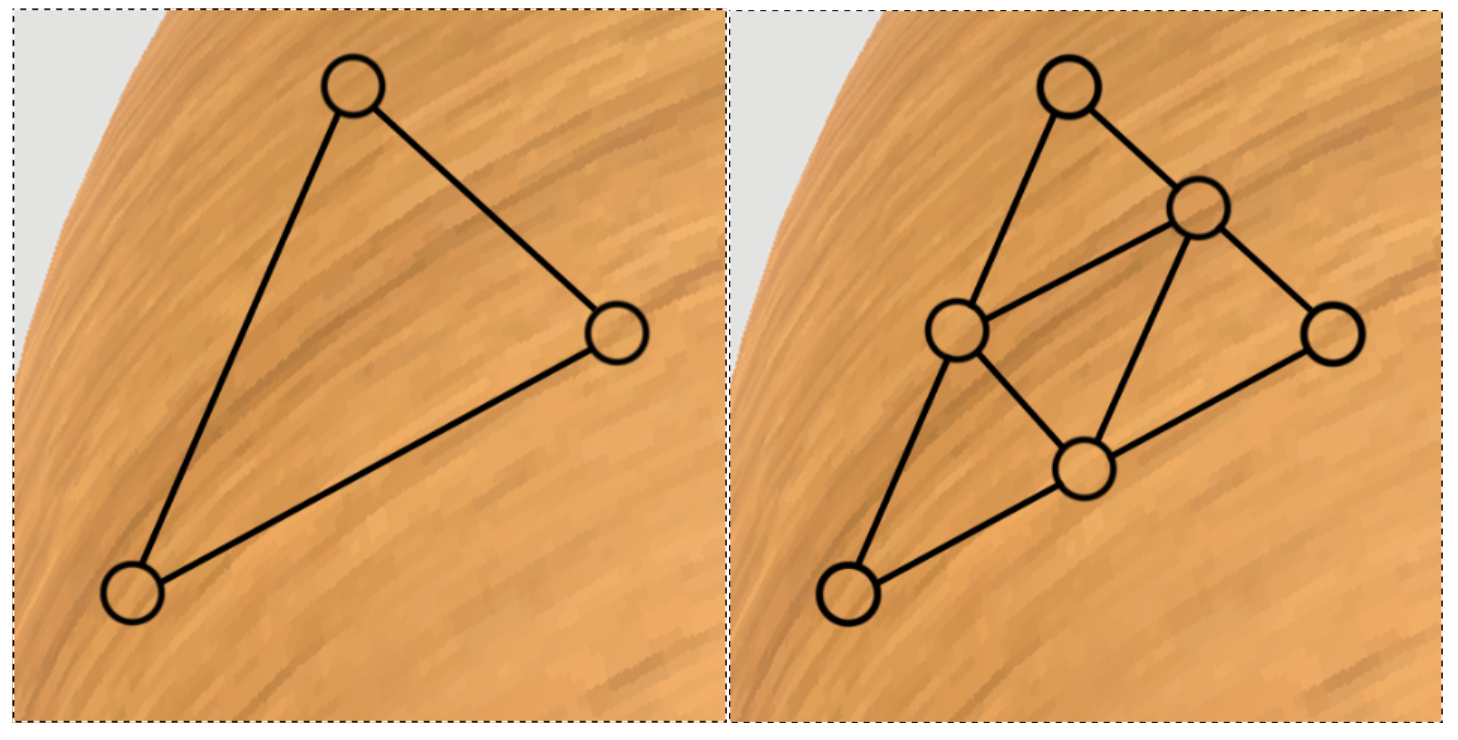
\includegraphics[width=0.9\linewidth]{figures/figure_mc.png}
\caption{The cameras configuration of our system. The different colors of point clouds shows the view of every cameras.}
\label{fig:camera_config}
\end{figure}

\subsubsection{Software}

OpenCV was used for camera calibration. CUDA was used for image processing and the kernel algorithm. Unity3D was used to implement the high-level application. It fetched live reconstruction from the kernel and rendered it in HTC Vive. Python was used for audio transmission.

\subsection{Calibration}

\subsubsection{Calibration between Cameras}

The \emph{camera calibration module} in OpenCV was used to calibrate the cameras. Each pair of cameras took ten snapshots (1080p color images) of a glass-made flat checkerboard. Then, OpenCV aligned their coordinates ($SD < 1 pixel$).

\subsubsection{Calibration between HMD and Cameras}

The HTC Vive was calibrated by setting the original point in its software. We placed the original point of the camera coordinates at the same position by using the checkerboard. Hence, we aligned the HTC Vive with the cameras. This calibration is not necessarily accurate because the users can hardly perceive the error [xx].

\subsection{Preprocessing}

\subsubsection{Depth Processing}

The cameras acquired depth images of $640 \times 480$ pixels at 30 FPS. The Realsense D415 is based on binocular disparity. Thus, disparity values (instead of depth values) were used in the processing for accuracy. We applied median filtering, spatial filtering, hole filling and temporary filtering on the depth images.

\subsubsection{Color Processing}

The cameras acquired color images of $960 \times 540$ pixels at 30 FPS. The exposure settings were manually adjusted. We used one RGB camera as the reference and matched the other cameras to this reference by white balancing and linear mapping.

\subsubsection{Background Removal}

The system can remove unnecessary background and retain only the individuals and the task objects. In the calibration step, we recorded the background as RGBD images. At runtime, we removed pixels that are similar to the background based on thresholds.

\subsection{3D Reconstruction}

We developed a real-time CUDA implementation of 3D reconstruction similar to KinectFusion \cite{izadi2011kinectfusion}. First, the algorithm integrated depth images into a TSDF Volume \cite{curless1996volumetric}. Next, the 3D mesh was extracted from the TSDF Volume using Marching Cubes \cite{lorensen1987marching}. Then, the algorithm projected color images on the 3D mesh for colorization.

The resolution of TSDF volume was $256 \times 256 \times 256$ voxels. In the TSDF processing, we used a weighted average where $W = \frac{1}{Dist}$ on different cameras to minimize the error. In the colorization, each triangle was upsampled to four quartered parts to sample more colors, because the users are more sensitive to the texture but not the shape \cite{sander2001texture}.

\subsection{The support of co-presence}

\subsubsection{Low network delay}

Figure \ref{fig:system_delay} shows the pipeline of our system. The one-way end-to-end delay was 52 ($\pm$ xx) ms, i.e., the time interval between a user acts and his partner sees. The frame rate of 3D reconstruction was 30 FPS. It was restricted by the frequency of Realsense. On average, a frame (33 ms) consisted of 19 ms processing and 14 ms idling. The remote images had one frame of latency. So the end-to-end delay was about $33 + 19 = 52$ ms. The rendering and the audio transmission were independent to the reconstruction pipeline. The frame rate of rendering reached 90 FPS so that the users do not feel dizzy. The audio channel was synchronized with the video channel by appending extra latency.

\begin{figure}[!htbp]
\centering
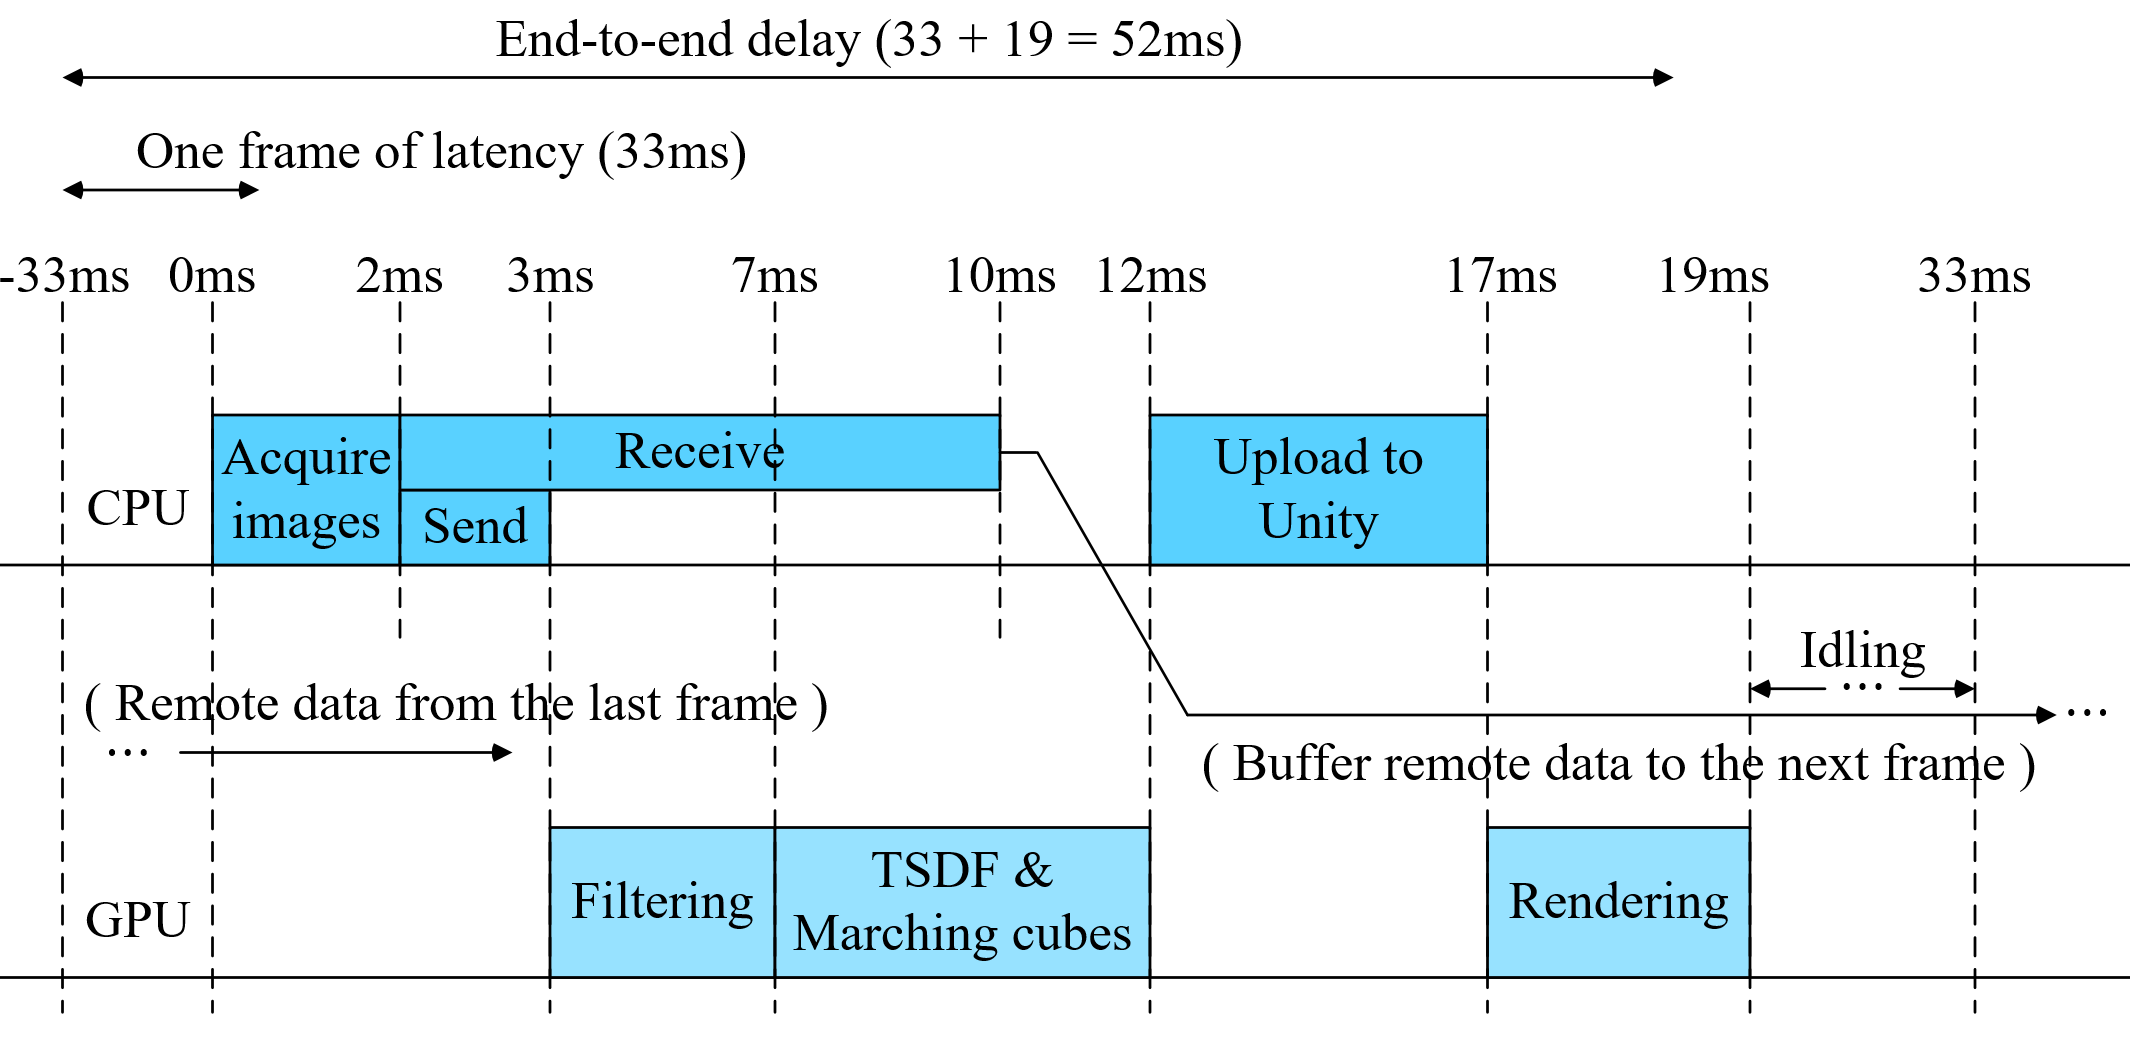
\includegraphics[width=1.0\linewidth]{figures/figure_pipeline_new3.png}
\caption{The pipeline.}
\label{fig:system_delay}
\end{figure}

We reached the high synchronicity by appropriate hardware, efficient GPU implementation and the only one frame of latency. The bottleneck of our pipeline is that Realsense limits a frame to be 33 ms. Another problem is that additional time is wasted in copying data to Unity3D. While Unity3D is important for the easy development, it only receives data through CPU codes, which wastes 5 ms per frame. This problem is possible to be refined in the future.

\subsubsection{Sync assistance}

For the tasks with a very high synchronicity requirement, we propose an assistant design to help synchronizing the task. While the transmission delay of data is unavoidable, it is possible to synchronize the time of two systems with almost zero milliseconds apart (the NTP protocol \cite{mills1991internet}). Thus, it is possible to provide zero-delay cues for the users in the two ends.

Take the Rock-Paper-Scissors game as example, we designed an audio source of "tick, tick, tack". The audio sources are played simultaneously in the two ends. The two users can show the gesture when they hear the "tack" sound. We assessed the effect of this design on user experience in the experiment.

\subsubsection{Shared space}

The system reconstructs physical scene in full 3D and renders it in head-mounted displays. It naturally supports that multiple users feel like locating at the same space.

\subsubsection{Shared props}

For two similar objects from the two ends, our system fuse their common parts together and retain their distinct parts. To create a shared prop, we first map their locations. If the scene contains only one shared prop, we can simply set the location of each physical prop as the origin point of each end. Otherwise we have to move the props to the same location in the virtual space manually. Then, our system merges the shared props automatically.

We modified the TSDF algorithm to merge the shared props. The merging rule is (see more information in \cite{curless1996volumetric}):
\begin{equation}
V_z=\min\{\frac{\sum_{local} W_{i,z}S_{i,z}}{\sum_{local} W_{i,z}},\frac{\sum_{remote} W_{j,z}S_{j,z}}{\sum_{remote} W_{j,z}}\}
\end{equation}
\begin{equation}
W_{i,z}=\frac{1}{dist(i,z)}    
\end{equation}
where $S_{i,z}$ is the Signed Distance Function (SDF) value of the $z$th volume from the $i$th camera. $dist(i,z)$ is the distance from the $i$th camera to the $z$th volume. $V_z$ is the merged SDF value of $z$th volume after the combination.

\begin{figure}[!htbp]
\centering
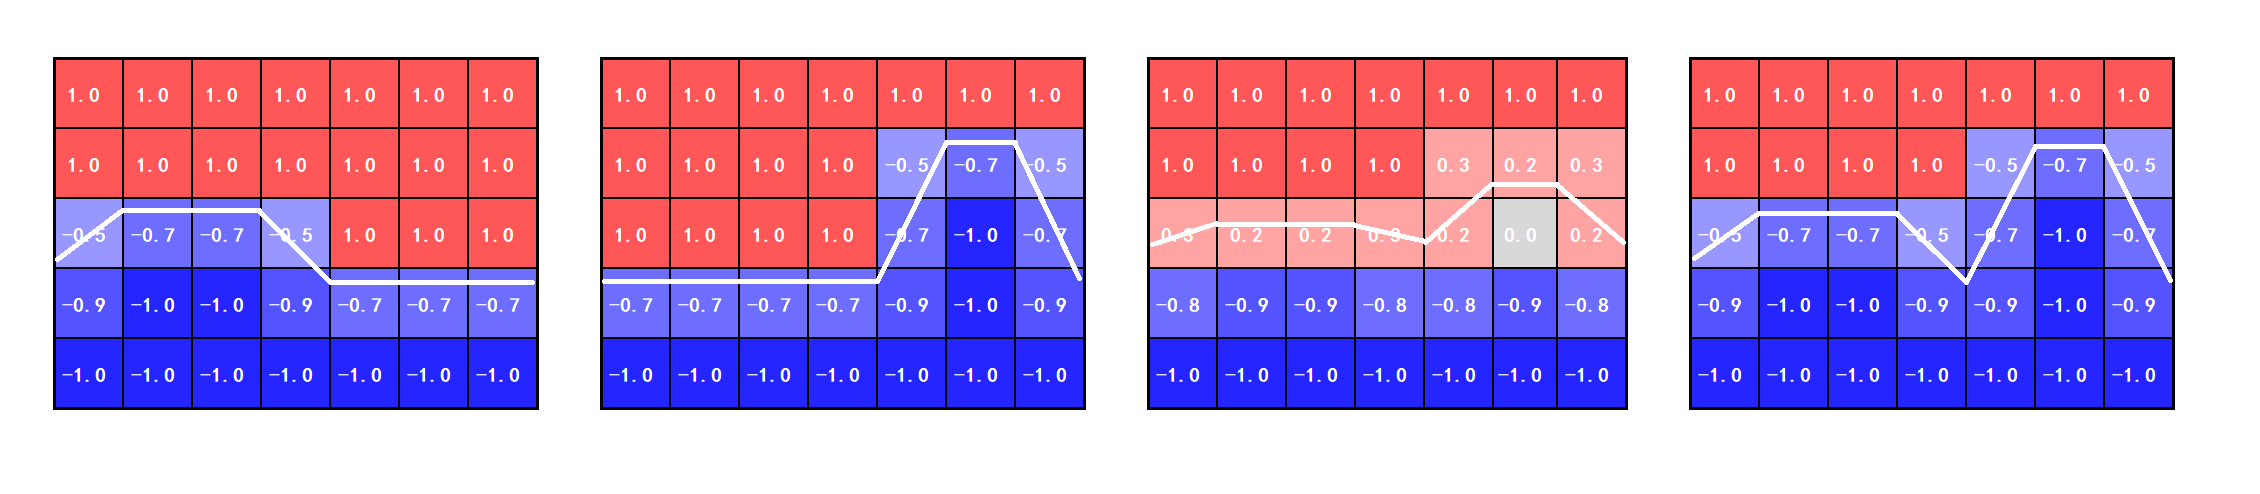
\includegraphics[width=1.0\linewidth]{figures/figure_tsdf.png}
\caption{Left to right: (1 \& 2) SDF values from cameras in the two ends 1; (3) Merged SDF value in a standard TSDF method; (4) Merged SDF value in our framework.【周诚驰】改进merge算法以后,拍两张只有黑棋和只有白棋的特写,再截一张效果图。}
\label{fig:TSDF_merge_two_sides}
\end{figure}

Figure \ref{fig:TSDF_merge_two_sides} shows the weighted combination of the two profile from both ends.


\section{User Experiment}

There are two motivations behind our study: first, we use this experiment to explain the four synchronization levels in our framework; second, we illustrate how to measure the noticeable delay and the acceptable delay for a specific application. The experiment is divided into two parts: playing chess and a the Rock-Paper-Scissors game.

\subsection{Part A: Playing Chess}



\subsection{Part B: Rock-Paper-Scissors}

[NOTE] a within study to test the four synchronization levels in our systems. 15 couples, with a total of 30 people take part in. Each participant tries all tasks, we used Latin square to balance the learning effect. For each task, participants had 5 sessions with different end-to-end delay, each of which was followed by short surveys asking participants to rate the experience. The motivation of this study is to investigate noticeability and annoyance of delay in various tasks. 

\subsection{Participants}

[NOTE] A couple of users know each other because they are friends, classmates or something else. User information like age, from campus, payment, whether familiar with AR/VR and telepresence or not.

[NOTE] Our first language is Chinese. This should be claimed because it affects conversion turn talking model. Native Chinese speaker

\subsection{Procedure}

[NOTE] Something the describe the experimental procedure.

After each session we assessed subjective feedback via questionnaires as Table \ref{tab:table_questionnaire} shown. Each session of questions includes perceived quality, noticeability and disruptiveness of delay.

\subsection{Results}

\subsection{NOTE: user experiment}

(PART A) control study for level 2, 3, 4

Duration: 1 hour

3 Tasks (Session) * 5 Delays (Trial)

Tasks = [Audiovisual Playing Chess; Visual Playing Chess; Playing Chess without seeing the partner]

Delays = [100 ms, 200 ms, …, 500 ms]

2 minute for each Trial

1 minute break and questionnaire between Trials

Questions:

(1) Quality: Excellent 1 <—> 5 Bad

(2) Noticeability: Not at all <—> Very much

5 minute break and interview between Sessions

Interview:

(1) How do you notice the delay? What is the cues?

(2) What make you intolerable in the task?

(3) Any commends?

(PART B) control study for level 1

(1) Level 1 (Forced Synchronization Interaction) is with high delay requirement.

(2) Visual assistance is a 0-delay visual cue for a pair to synchronize

Duration: 0.5 hour

2 Tasks * 2 Conditions * 3 Delays

Tasks = [Rock-paper-scissors, counting down]

Conditions = [with, without visual assistance]

Delays = [100 ms, 150 ms, 200 ms]

2 minute for each trial (including questionnaire and rest)

5 minute break and interview between Sessions

\section{Literature Review and Background}

3D telepresence requires three processes: reconstruction, transmission and rendering \cite{fuchs2014immersive}. In this section, we first review 3D reconstruction techniques. Parallel computing becomes important for a real-time high-quality reconstruction. Then, we discuss the transmission requirement of network delay by reviewing delay perception in tele-communication. Last, we analyze the sense of immersion supported by different display devices. We recommend Head-Mounted Display (HMD) as a practical approach to support a high level of immersion.

%We do not focus on transmission techniques as \cite{beck2013immersive, pece2011adapting} did, but use a 10 Gigabit Ethernet connection

% We used TSDF Volume \cite{curless1996volumetric} and Marching Cubes \cite{lorensen1987marching} for reconstruction, a 10 Gigabit Ethernet connection for transmission, and Unity3D for rendering in HTC Vive.

% A 3DTI system requires three processes: reconstruction, transmission and rendering \cite{fuchs2014immersive}. For reconstruction, volumetric methods have become mainstream, e.g., Truncated Signed Distance Function (TSDF) Volume \cite{curless1996volumetric}, Marching Cubes \cite{lorensen1987marching} and Fusion4D \cite{dou2016fusion4d}. Our system does not focus on transmission as \cite{beck2013immersive, pece2011adapting} did, but uses a direct Ethernet connection instead. For rendering, we recommend Head-Mounted Display (HMD) because it supports co-presence.

\subsection{3D Reconstruction}

In the late 20th century, 3D reconstruction was either an off-line concept \cite{lorensen1987marching, curless1996volumetric} or simple polygonal models that look correct \cite{kanade1997virtualized, fuchs1994virtual, gibbs1999teleport}. In the early 21st century, researchers achieved quasi real-time methods based on point cloud \cite{gross2003blue, towles20023d} and triangulation \cite{kurillo2008immersive, petit2010multicamera, maimone2011encumbrance}.

In the past decade, parallel computing devices (e.g., GPUs) became powerful. 3D reconstruction reached the real-time performance \cite{maimone2012real, loop2013real} through volumetric methods that work in parallel. Microsoft's KinectFusion \cite{izadi2011kinectfusion} is a representative work. They described a GPU-based pipeline that generates high-quality 3D models in real time. Much previous work focused on improving 3D reconstruction within the framework of KinectFusion in regions of scale \cite{niessner2013real, chen2013scalable}, noise reduction \cite{khoshelham2012accuracy, nguyen2012modeling, newcombe2015dynamicfusion} and so on.

% [paragraph] toward fusion4D and its drawback (2016)
In 2016, Microsoft proposed the state-of-the-art pipeline named Fusion4D \cite{dou2016fusion4d}, which is highly robust to occlusions, large frame-to-frame motions, and topology changes. The fourth dimension is time, indicating that it leverages inter prediction. In the same year, Microsoft integrated fusion4D into their 3D telepresence system Holoportation \cite{orts2016holoportation}. However, Holoportation is expensive, not open-source and not responsive enough. Our framework applies a 3D reconstruction method similar to KinectFusion \cite{izadi2011kinectfusion}, which is based on Truncated Signed Distance Function (TSDF) Volume \cite{curless1996volumetric} and Marching Cubes \cite{lorensen1987marching}.

\subsection{Delay perception in tele-communication}

Network delay is a crucial factor that affects user experience in tele-communication \cite{brunnstrom2013qualinet, schmitt2013qoe, wu2009quality}. Numerous studies have been carried out to explore delay perception in telephone and 2D tele-communication.

%The noticeability of network delay and the overall rating of network quality are two important factors measured by most studies \cite{geerts2011we, schmitt2014asymmetric, schmitt2014influence, wu2009quality}.

For audio-medicated communication, one-way delay of 150 ms has become a standard for good user experience \cite{recommendation2003114}. \cite{gergle2006impact} summarized prior works on audio delay and found that delays below 300 ms pose little problem, while delays above 450 ms can severely impact communication.

For 2D tele-communication, \cite{tam2012video, polycom2006traffic} reviewed prior works and found that one-way delays would be noticeable between 100 and 150 ms. Compared to the audio-medicated communication, delay had a weaker impact on naturalness when both audio and video channels were available \cite{tam2012video}.

% [paragraph] existing work of delay perception in 3DTI
For 3D telepresence, negative impacts of large network delay are widely reported \cite{beck2013immersive, gibbs1999teleport, maimone2011encumbrance, kurillo2008immersive, raghuraman2015distortion}. A few works studied delay perception in 3D telepresence \cite{wu2010m, huang2012towards, wu2009quality}. \cite{wu2009quality} conducted a study in a simple 3D telepresence system that renders live reconstruction in 2D screen. They found that an one-way network delay of 120 ms can be predictable and disruptive in their system. To our knowledge, no work has been done to study delay in 3D telepresence with a high level of co-presence. It is unknown whether the standard of 100 ms to 150 ms is enough in 3D.

\subsection{3D Rendering}

Human sense the 3D environment by four types of cues: pictorial depth cues, motion parallax, binocular vision and accommodation \cite{kooi2004visual}. Different display devices support different levels of 3D perception. For examples, 2D screens provide pictorial depth cues; head-tracked auto-stereo displays \cite{maimone2011encumbrance, maimone2012real, pejsa2016room2room} support pictorial depth cues and motion parallax.

Light field displays \cite{jones2007rendering, jurik2011prototyping, kim2012telehuman, gotsch2018telehuman2} can fully support the sense of 3D. However, they suffer from low resolution because of the huge computation. Most practical 3D displays support pictorial depth cues, motion parallax and binocular vision, but not accommodation. Spatially Immersive Displays (SIDs) and Head-Mounted Displays (HMDs) are the two typical techniques.

% Pictorial depth cues can provide 3D perception with one eye, .e.g., cast shadows and occlusion. Motion parallax is that the user can change his point of view and direction of gaze naturally in a 3D environment \cite{fuchs2014immersive}. Binocular vision is that human can perceive depth by the slightly different location of the left and right eyes. Accommodation is the automatic adjustment of the focus of the eye. Table xxx shows how existing display devices support these cues.

Around year 2000, SIDs had become increasing significant \cite{gross2003blue}. CAVE \cite{cruz1993surround} is a typical SID system that consists of surround-screen projection. Most 3D telepresence systems at that time applied rendering techniques similar to CAVE \cite{gibbs1999teleport, towles20023d, kurillo2008immersive, benko2012miragetable}. Latter researchers improved SIDs by supporting multi-user \cite{frohlich2005implementing, kulik2011c1x6, guan2018two} and glasses-free experience \cite{benko2014dyadic, jones2014roomalive, pejsa2016room2room}.

% However, SIDs can not support co-presence because there is an unavoidable 'window' that separates users into two virtual spaces.

Recently, HMDs become popular. More 3D telepresence systems tend to apply HMDs for 3D rendering \cite{orts2016holoportation, maimone2013general, lindlbauer2018remixed, smith2018communication}. HMDs are basically cheaper and easier to deploy compared to SIDs. There are two categories of HMDs: Virtual Reality (VR) and Augmented Reality (AR). Remixed Reality \cite{lindlbauer2018remixed} suggests that we can leverage both the benefits of AR and VR by rendering live 3D reconstruction in VR.

% Another superiority of HMDs is the ability to support co-presence \cite{maimone2013general, orts2016holoportation}.

%\subsection{Media Richness in 3DTI}

%Media richness theory suggests that communication with rich media information can help reduce uncertainty and equivocality \cite{daft1986organizational}. Media richness is defined as the potential information carrying capacity of data. Different media have varied richness and can be determined by three factors: immediate feedback capacity, multiple cues and language restriction \cite{daft1983information}. Face-to-face communication is the richest form of information processing. It provides immediate feedback, contains multiple cues such as audio and visual information and is the most natural way of human communication. 

%The theory can be applied to 3DTI study as well. Previous work in building 3DTI system focused mainly on rendering quality of visual space \cite{kurillo2008framework, kurillo2008immersive}.  However, we argue that in addition to vision, there are also other important factors that contribute to good quality of user experience, such as audio, tactility and co-presence. Audio and tactile sense extends the potential information carried by data transmission, which users can use to reduce uncertainty and correct misunderstanding instantly. Meanwhile, co-presence enables two users feel like they were having a face-to-face communication and would probably improve quality of user experience. We believe a good 3DTI system should be developed upon a rich set of media information with all these factors taken into consideration.



\section{Limitation}

1. The rendering quality of the system is not state-of-the-art.

2. The lack of eye contact.

3. The low external validity of the experiment.


\section{Conclusion}

This paragraph is for the conclusion.

\begin{acks}

We thank all the volunteers, and all publications support and staff, who wrote and provided helpful comments on previous versions of this document. Authors 1, 2, and 3 gratefully acknowledge the grant from NSF (\#1234--2012--ABC). \textit{This whole paragraph is just an example.}

\end{acks}

\bibliographystyle{ACM-Reference-Format}
\bibliography{bibliography}

\end{CJK*}

\end{document}
